\documentclass[aspectratio=169,hyperref={pdfpagelabels=false}]{beamer}
\input{preamble.tex}

\subtitle{\normalsize{Industrial IoT for Digitization of Electronis Assets}}
\title{}

\setdepartment{DTU Wind and Energy System}
\setcolor{blue}

\begin{document}
\inserttitlepage

%B SLIDE 0
\begin{frame}{Agenda}
  \tableofcontents
\end{frame}

% SLIDE 1
\begin{frame}{}

  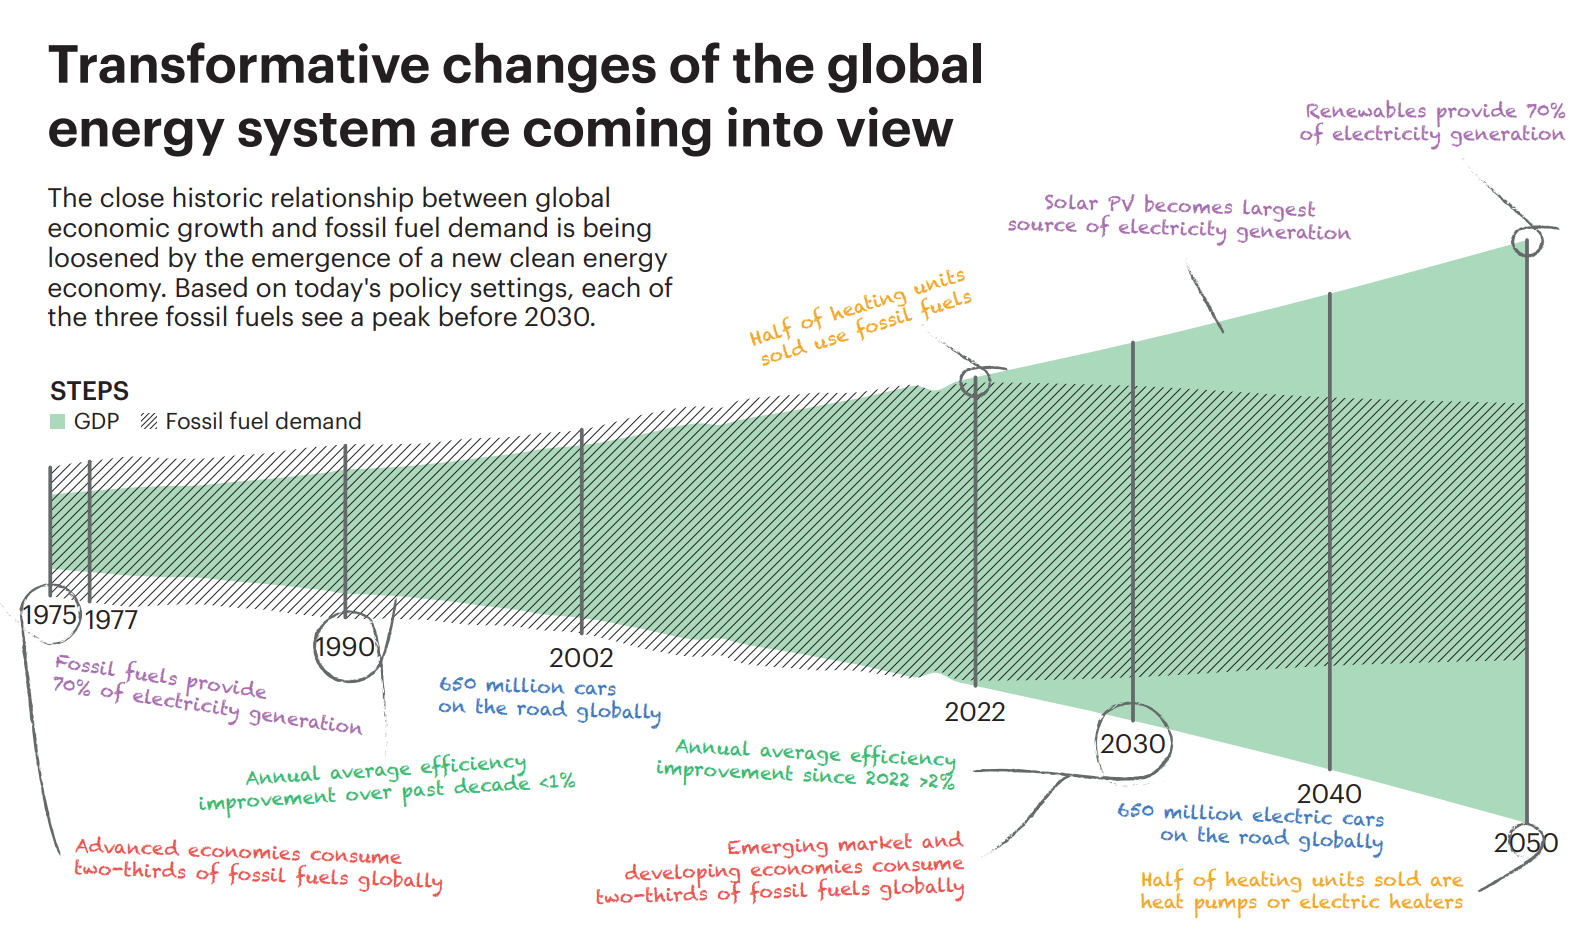
\includegraphics[width=0.9\textwidth]{img/pic0.png} 
      \footnotetext{World Energy Outlook 2023, iea}
    \end{frame}

% SLIDE 2
    \begin{frame}{The Green Transition and European Targets}
    Europe has set the goal of reducing 40\% of Greenhouse Gas emissions by 2030 and the 80-95\% by 2050, to reach the target of maintaining global atmospheric warming below the 2°C. 
    To accomplish this target, massive investment in renewables is on the way:

    \vspace*{1em}

        \begin{columns}
      
          % Left column
          \begin{column}{0.4\textwidth}
            % Add your text here
            \textbf{Key Goals: }
            \begin{itemize}
                \item[-] 45\% of Renewables by 2030
            \end{itemize}
            \begin{itemize}
                \item \textbf{600 GW} of Solar Capacity
                \item \textbf{450 GW} of Wind Capacity
            \end{itemize}
            
          \end{column}
      
          % Right column
          \begin{column}{0.7\textwidth}
            % Add your image here
            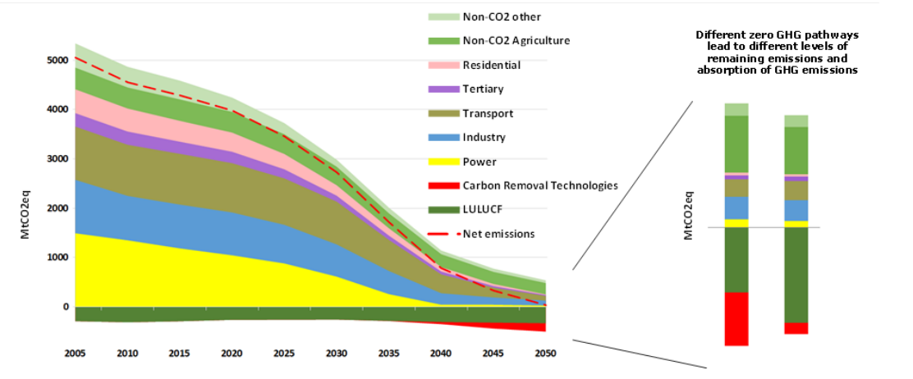
\includegraphics[width=\textwidth]{img/pic1.png} % Replace with your image path
          \end{column}
        \end{columns}
        \footnotetext{European policies on climate and energy towards 2020, 2030 and 2050}
      \end{frame}

% SLIDE 3
\begin{frame}{Future Projections In Denmark}

        \begin{columns}
          % Left column
          \begin{column}{0.4\textwidth}
            Word leading country in wind energy with more than 44\% of the energy production from renewable sources.
            Carbon Neutral by 2030, with Offshore and Onshore Wind up to 13 GW and Solar up to then 10 GW.
            
          \end{column}
      
          % Right column
          \begin{column}{0.5\textwidth}
            % Add your image here
            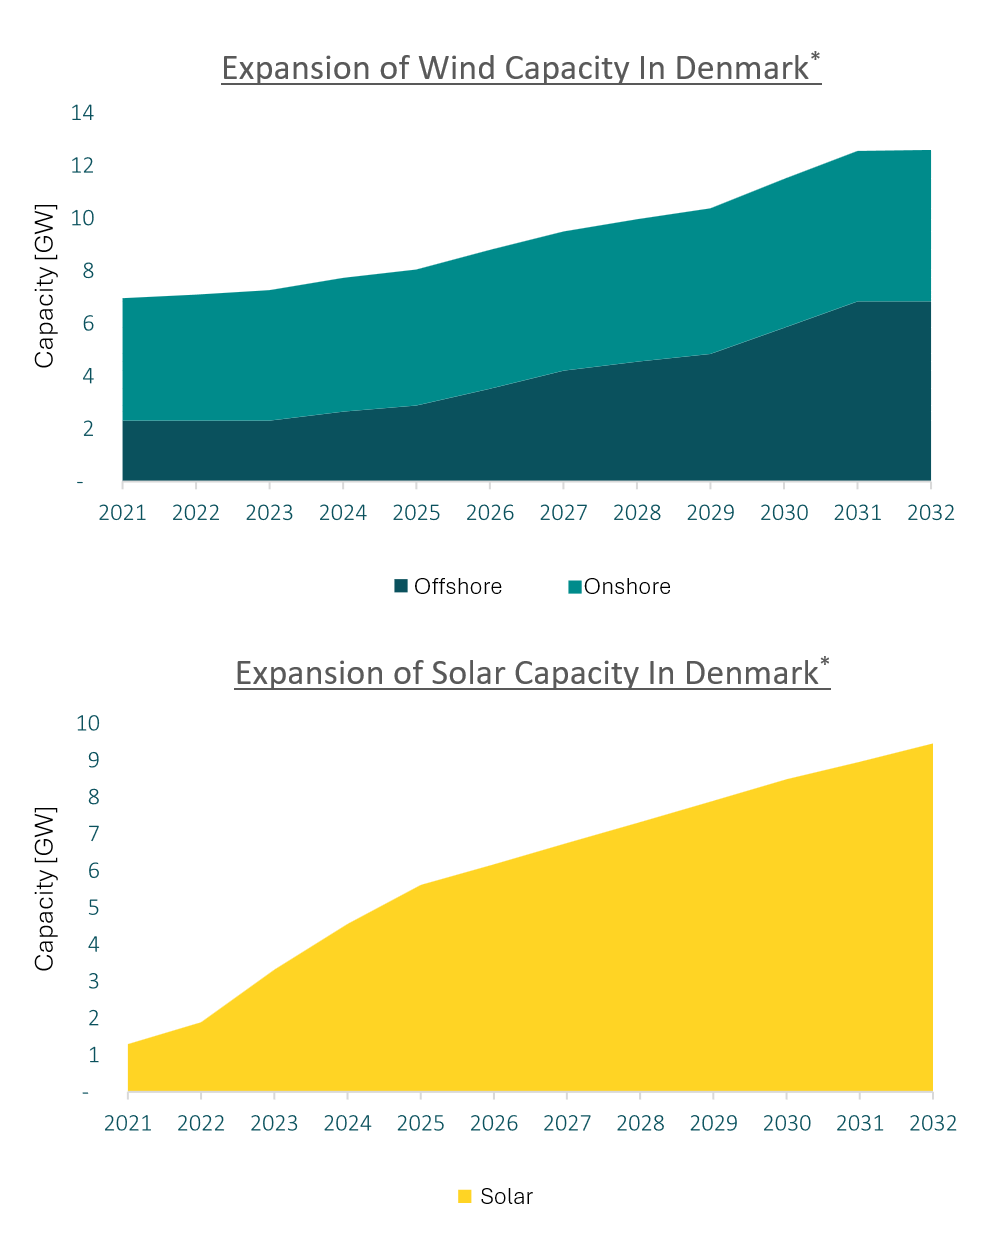
\includegraphics[width=0.75\textwidth]{img/pic2.png} % Replace with your image path
          \end{column}
        \end{columns}
        \footnotetext{Energinet. (2022). SCENARIERAPPORT 2022 – 2032: Forventninger til fremtidens Systemydelser. Energinet}
      \end{frame}

% SLIDE 4
\begin{frame}{Main Challenges of energy sistem based on Renewables}

\includegraphics[width=0.3\textwidth]{img/pic5.png} \centering
\end{frame}
        
% SLIDE 5
\begin{frame}{Past and Future Challenges}
  \begin{columns}
    % Left column
    \begin{column}{0.5\textwidth}
      \begin{itemize}
        \item Higher chance of frequency events. 
        \item Higer capacity of Ancillary Services. 
        \item Tailored control strategies. 
        \item Reduce the curtailment of energy production with BESS. \pause
      \end{itemize}
    \end{column}

    % Right column
    \begin{column}{0.5\textwidth}
      \begin{itemize}
        \item Exploit flexibility of variable loads (\textit{fans, drives, compressors}). 
        \item Aggregate multiple presumers.
        \item Data-driven modeling solutions. 
        \item Bosting digitalization of old assests. 
      \end{itemize}
    \end{column}
  \end{columns}
\end{frame}

% SLIDE 5
\begin{frame}{Digital Twins: \\ \vspace{0.5em}
               \normalsize{A core technology to boost the Digitalization}}

  \begin{figure}[h]
    \vspace{3em}
    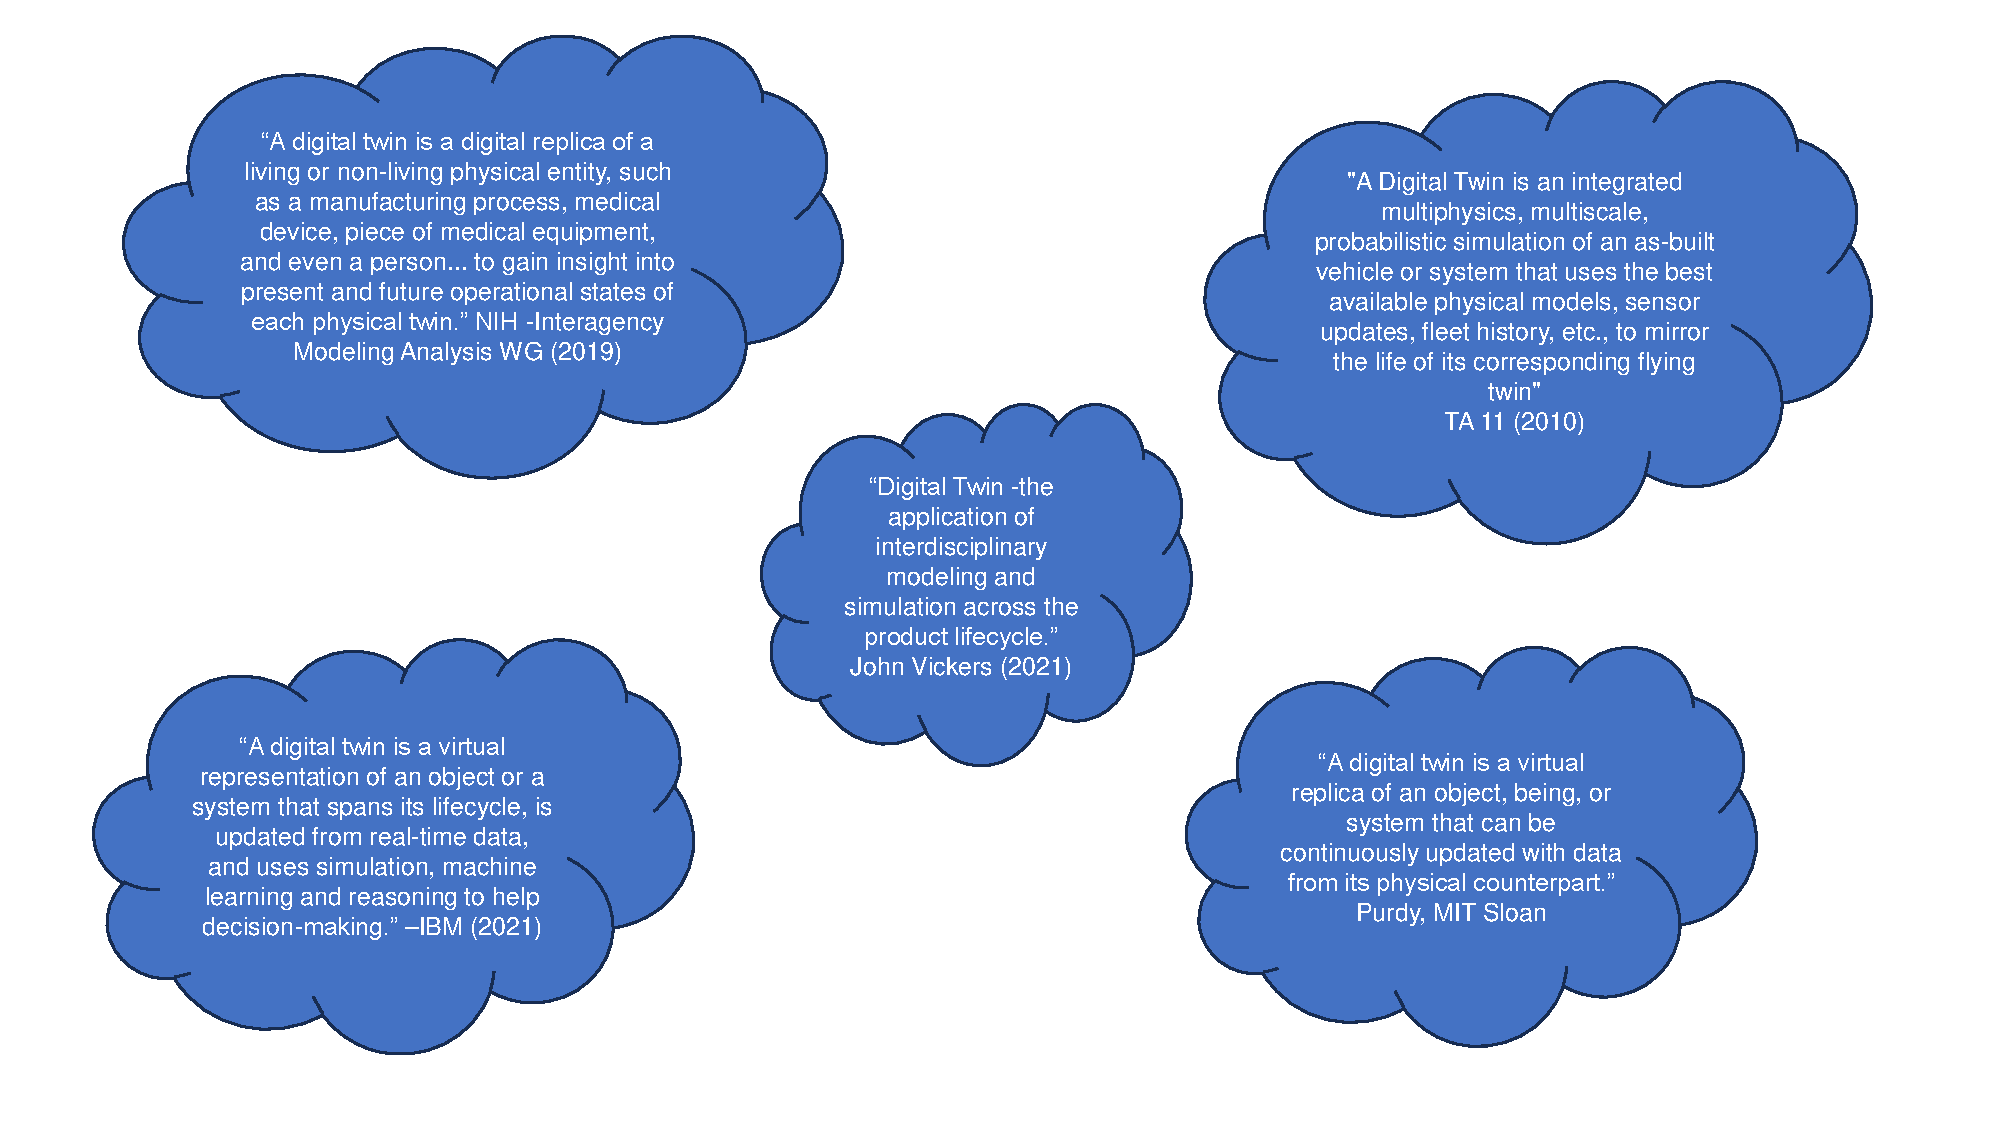
\includegraphics[width=0.85\textwidth]{img/digital_twin_definitions.pdf} \centering
  \end{figure}
\end{frame}

% SLIDE 6
\begin{frame}{Digital Twins: \\ \vspace{0.5em}
  \normalsize{A core technology to boost the Digitalization}}
\begin{figure}[h]
  \vspace{1em}
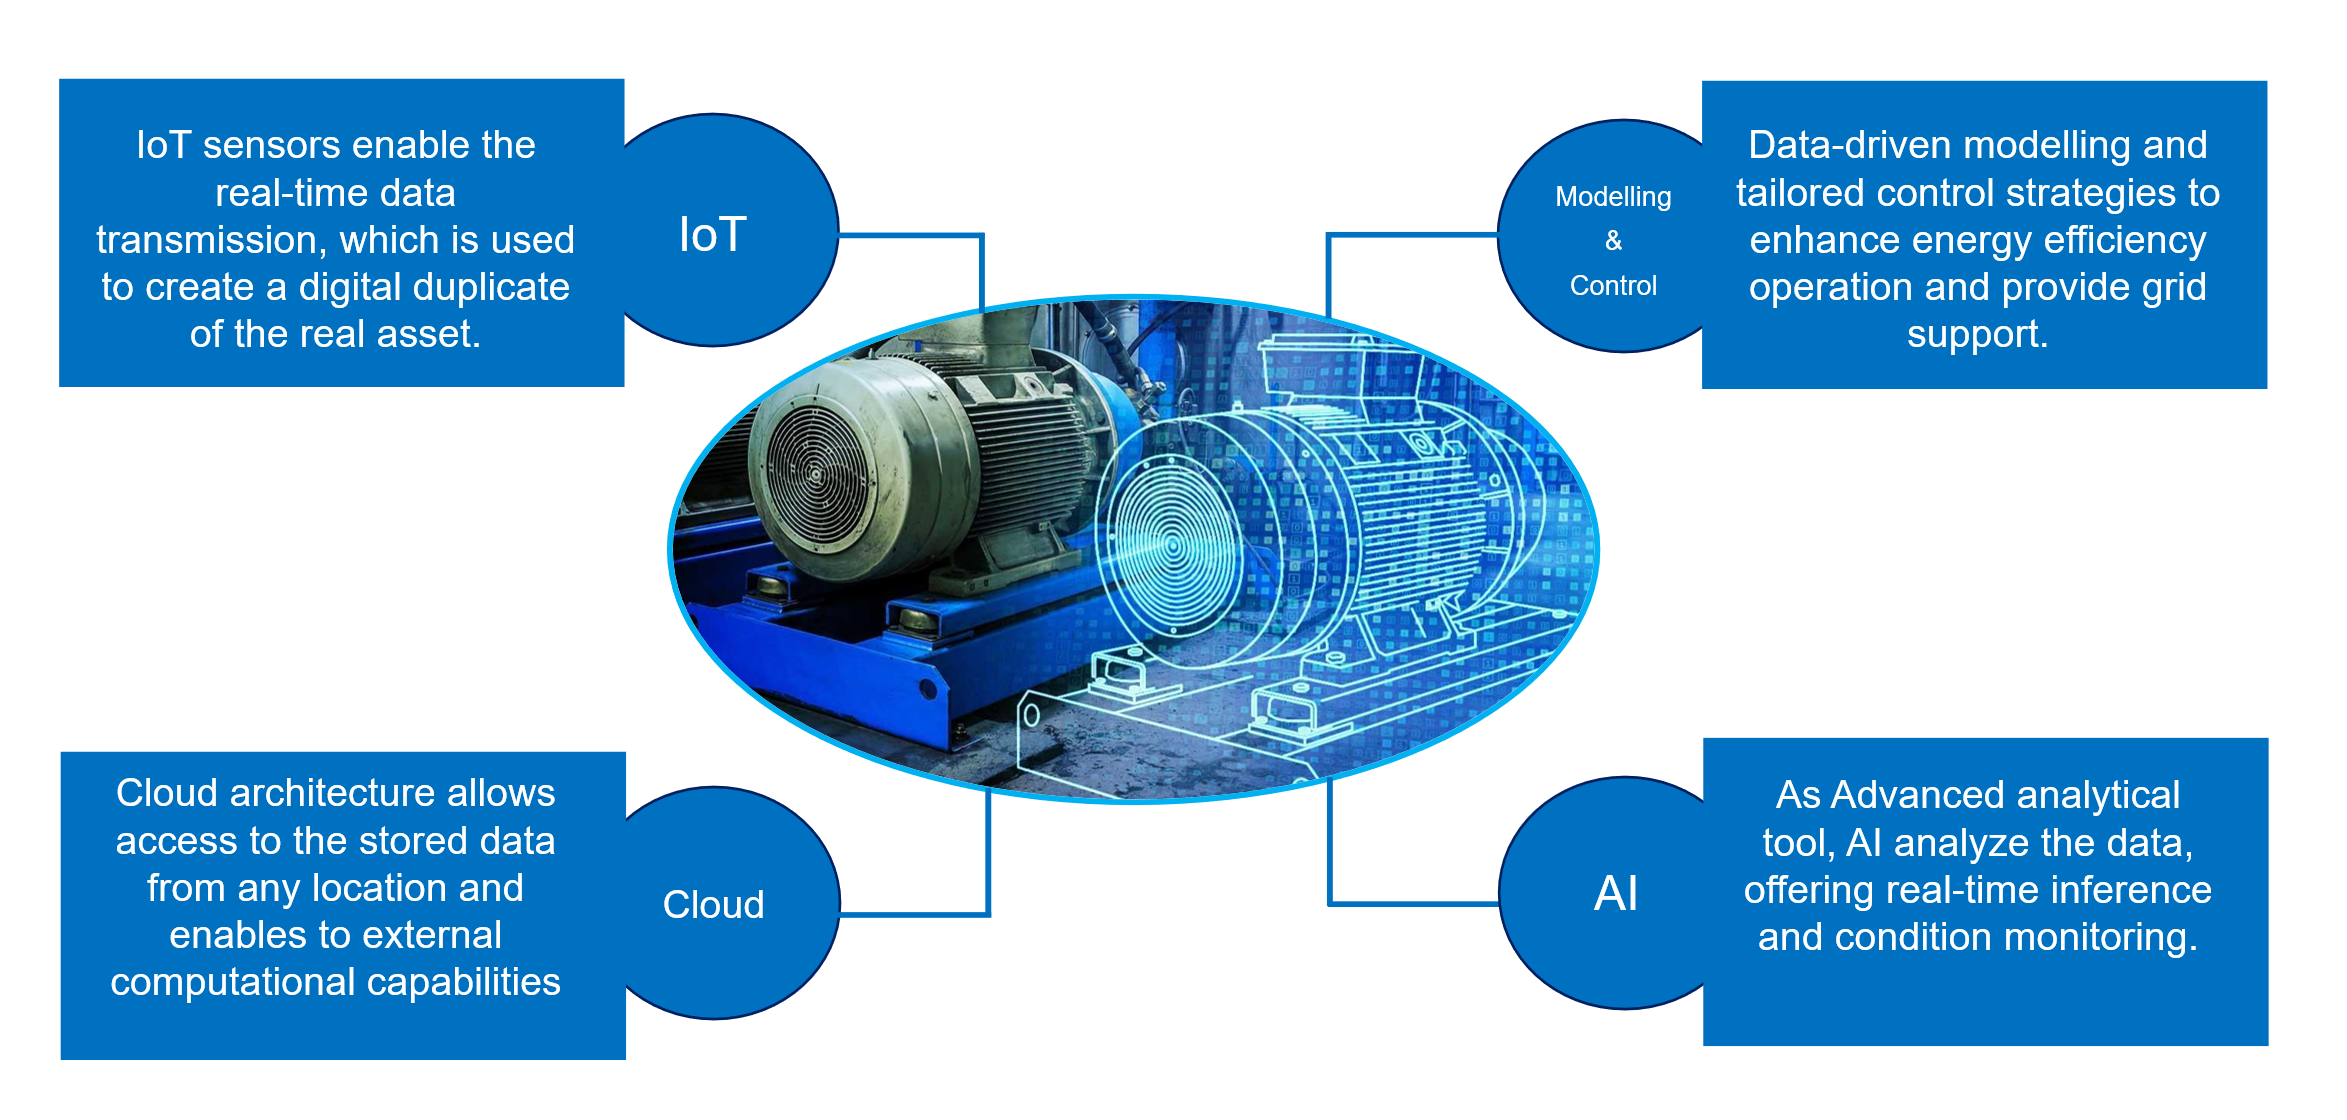
\includegraphics[width=1.05\textwidth]{img/pic7.png} \centering
\end{figure}
\end{frame}

\end{document}